\documentclass[
margin=2mm,
]{standalone}

\usepackage[utf8]{vietnam}
\usepackage{times}
\usepackage{pgfplots}
\usepackage{scrextend}
\changefontsizes{15pt}
\pgfplotsset{compat=1.18}
\usepackage{xcolor}
\usepackage{tikz}
\usepgfplotslibrary{groupplots}
\usetikzlibrary{arrows.meta, positioning, shapes.multipart, fit}

\definecolor{CTUblue}{rgb}{0.121568627450,0.3607843137,0.662745098}
\definecolor{CTUcyan}{rgb}{0,0.6862745098,0.937254902}

\begin{document}
	
	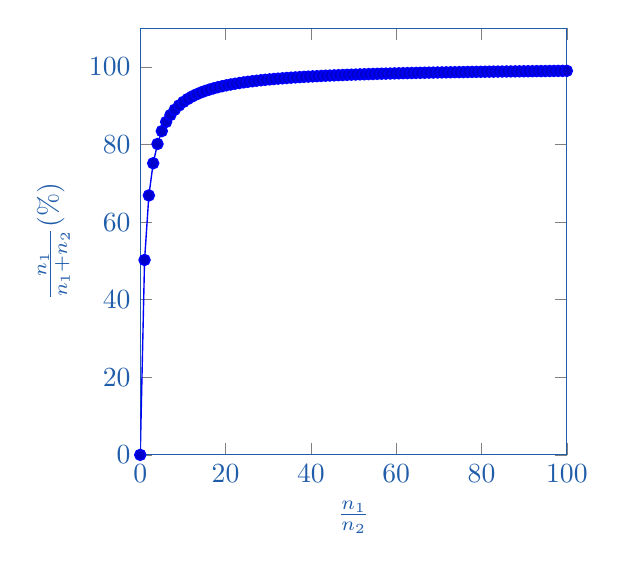
\begin{tikzpicture}
		\begin{axis}[
			width=7cm, height=7cm,
			xmin=0, xmax=100,
			ymin=0, ymax=110,
			axis lines=box,
			CTUblue,
			xlabel={$\frac{n_1}{n_2}$},
			ylabel={$\frac{n_1}{n_1+n_2} (\%)$},
			every axis plot/.append style={line width=0.5pt, color = CTUcyan,draw=CTUcyan},
			domain=0:100,
			samples=100,
			]
			% Hàm y = 1 - 1/(x+1)
			\addplot {(1 - 1/(x+1) )*100};

,		\end{axis}
	\end{tikzpicture}
	
\end{document}
